\section{系统详细设计}

	系统详细设计实现省略一段文字省略一段文字省略一段文字省略一段文字省略一段文字省略一段文字省略一段文字省略一段文字省略一段文字省略一段文字省略一段文字省略一段文字省略一段文字省省略一段文字省略一段文字省略一段文字省略一段文字省略一段文字省略一段文字省略一段文字省略一段文字省略一段文字省略一段文字省略一段文字省略一段文字省略一段文字省

  \subsection{基础层详细设计}
	
   	\subsubsection{网络通信的实现}

		实现省略一段文字省略一段文字省略一段文字省略一段文字省略一段文字省略一段文字省略一段文字省略一段文字省略一段文字省略一段文字省略一段文字省略一段文字省略一段文字省省略一段文字省略一段文字省略一段文字省略一段文字省略一段文字省略一段文字省略一段文字省略一段文字省略一段文字省略一段文字省略一段文字省略一段文字省略一段文字省

		
		这里以\Cref{code_api_service} 为例,代码块使用示例
		
		
		\begin{lstlisting}[caption=APIService , label=code_api_service]
 /** 
  * 登录 
  */
 @POST("user/login")
 Call<APIResponse<LoginResponse>> login(@Body LoginRequest request);

 /** 
  * 获取单个用户详细信息
  */
 @GET("user/{imid}/info")
 Call<APIResponse<UserInfo>> getUserInfo(@Path("imid") String imId);
 
		\end{lstlisting}                 

	
			
   	\subsubsection{日志记录的实现}
    
    实现省略一段文字省略一段文字省略一段文字省略一段文字省略一段文字省略一段文字省略一段文字省略一段文字省略一段文字省略一段文字省略一段文字省略一段文字省略一段文字省省略一段文字省略一段文字省略一段文字省略一段文字省略一段文字省略一段文字省略一段文字省略一段文字省略一段文字省略一段文字省略一段文字省略一段文字省略一段文字省日志记录输出样式如\Cref{img_log_sample}所示。
    
    \begin{figure}[H]
    	\centering
    	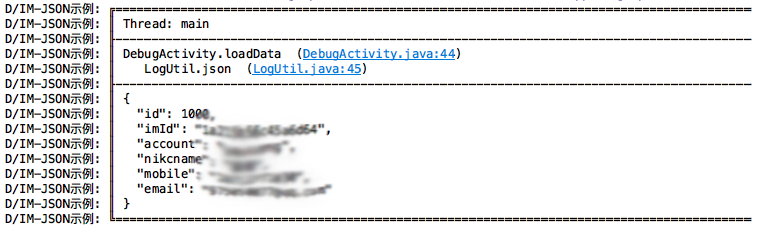
\includegraphics[width=0.95\textwidth]{images/log_sample}
    	\caption{日志信息示例}
    	\label{img_log_sample}
    \end{figure}
    
    
   	\subsubsection{加密解密的实现}
    
    实现省略一段文字省略一段文字省略一段文字省略一段文字省略一段文字省略一段文字省略一段文字省略一段文字省略一段文字省略一段文字省略一段文字省略一段文字省略一段文字省省略一段文字省略一段文字省略一段文字省略一段文字省略一段文字省略一段文字省略一段文字省略一段文字省略一段文字省略一段文字省略一段文字省略一段文字省略一段文字省
        
   	\subsubsection{缓存的实现}
   	
   	实现省略一段文字省略一段文字省略一段文字省略一段文字省略一段文字省略一段文字省略一段文字省略一段文字省略一段文字省略一段文字省略一段文字省略一段文字省略一段文字省省略一段文字省略一段文字省略一段文字省略一段文字省略一段文字省略一段文字省略一段文字省略一段文字省略一段文字省略一段文字省略一段文字省略一段文字省略一段文字省
   	   	
   	\subsubsection{文件操作工具的实现}
   	
   	文件操作模块定义了全局工具类 FileUtil,内部实现了常用的文件操作方法以及格式化输出文件大小的方法。常用文件操作方法包含判断文件是否存在、读文件、写文件、移动文件、复制文件、删除文件、创建文件、文件重命名、获取文件名称、判断是否有文件夹、调用系统方式打开文件、将字符串以不同形式的编码写入文件中。格式化文件大小主要是将文件的大小转换为更直观的形式,如:15KB、0.38M、1.52G。
   	
   	\subsubsection{JSON解析的实现}

	实现省略一段文字省略一段文字省略一段文字省略一段文字省略一段文字省略一段文字省略一段文字省略一段文字省略一段文字省略一段文字省略一段文字省略一段文字省略一段文字省省略一段文字省略一段文字省略一段文字省略一段文字省略一段文字省略一段文字省略一段文字省略一段文字省略一段文字省略一段文字省略一段文字省略一段文字省略一段文字省
	
  \subsection{数据层详细设计}

	实现省略一段文字省略一段文字省略一段文字省略一段文字省略一段文字省略一段文字省略一段文字省略一段文字省略一段文字省略一段文字省略一段文字省略一段文字省略一段文字省省略一段文字省略一段文字省略一段文字省略一段文字省略一段文字省略一段文字省略一段文字省略一段文字省略一段文字省略一段文字省略一段文字省略一段文字省略一段文字省
		 
	
	实现省略一段文字省略一段文字省略一段文字省略一段文字省略一段文字省略一段文字省略一段文字省略一段文字省略一段文字省略一段文字省略一段文字省略一段文字省略一段文字省省略一段文字省略一段文字省略一段文字省略一段文字省略一段文字省略一段文字省略一段文字省略一段文字省略一段文字省略一段文字省略一段文字省略一段文字省略一段文字省
	
	
  \subsection{组件层详细设计}

   	\subsubsection{二维码扫描的实现}
   	
	实现省略一段文字省略一段文字省略一段文字省略一段文字省略一段文字省略一段文字省略一段文字省略一段文字省略一段文字省略一段文字省略一段文字省略一段文字省略一段文字省省略一段文字省略一段文字省略一段文字省略一段文字省略一段文字省略一段文字省略一段文字省略一段文字省略一段文字省略一段文字省略一段文字省略一段文字省略一段文字省

   	\subsubsection{消息列表的实现}
	
	实现省略一段文字省略一段文字省略一段文字省略一段文字省略一段文字省略一段文字省略一段文字省略一段文字省略一段文字省略一段文字省略一段文字省略一段文字省略一段文字省省略一段文字省略一段文字省略一段文字省略一段文字省略一段文字省略一段文字省略一段文字省略一段文字省略一段文字省略一段文字省略一段文字省略一段文字省略一段文字省
	
   	\subsubsection{输入面板的实现}
   	
   	实现省略一段文字省略一段文字省略一段文字省略一段文字省略一段文字省略一段文字省略一段文字省略一段文字省略一段文字省略一段文字省略一段文字省略一段文字省略一段文字省省略一段文字省略一段文字省略一段文字省略一段文字省略一段文字省略一段文字省略一段文字省略一段文字省略一段文字省略一段文字省略一段文字省略一段文字省略一段文字省,输入面板具体样式如\Cref{input_panel}所示。
   	
   	\begin{figure}[H]
		\centering
		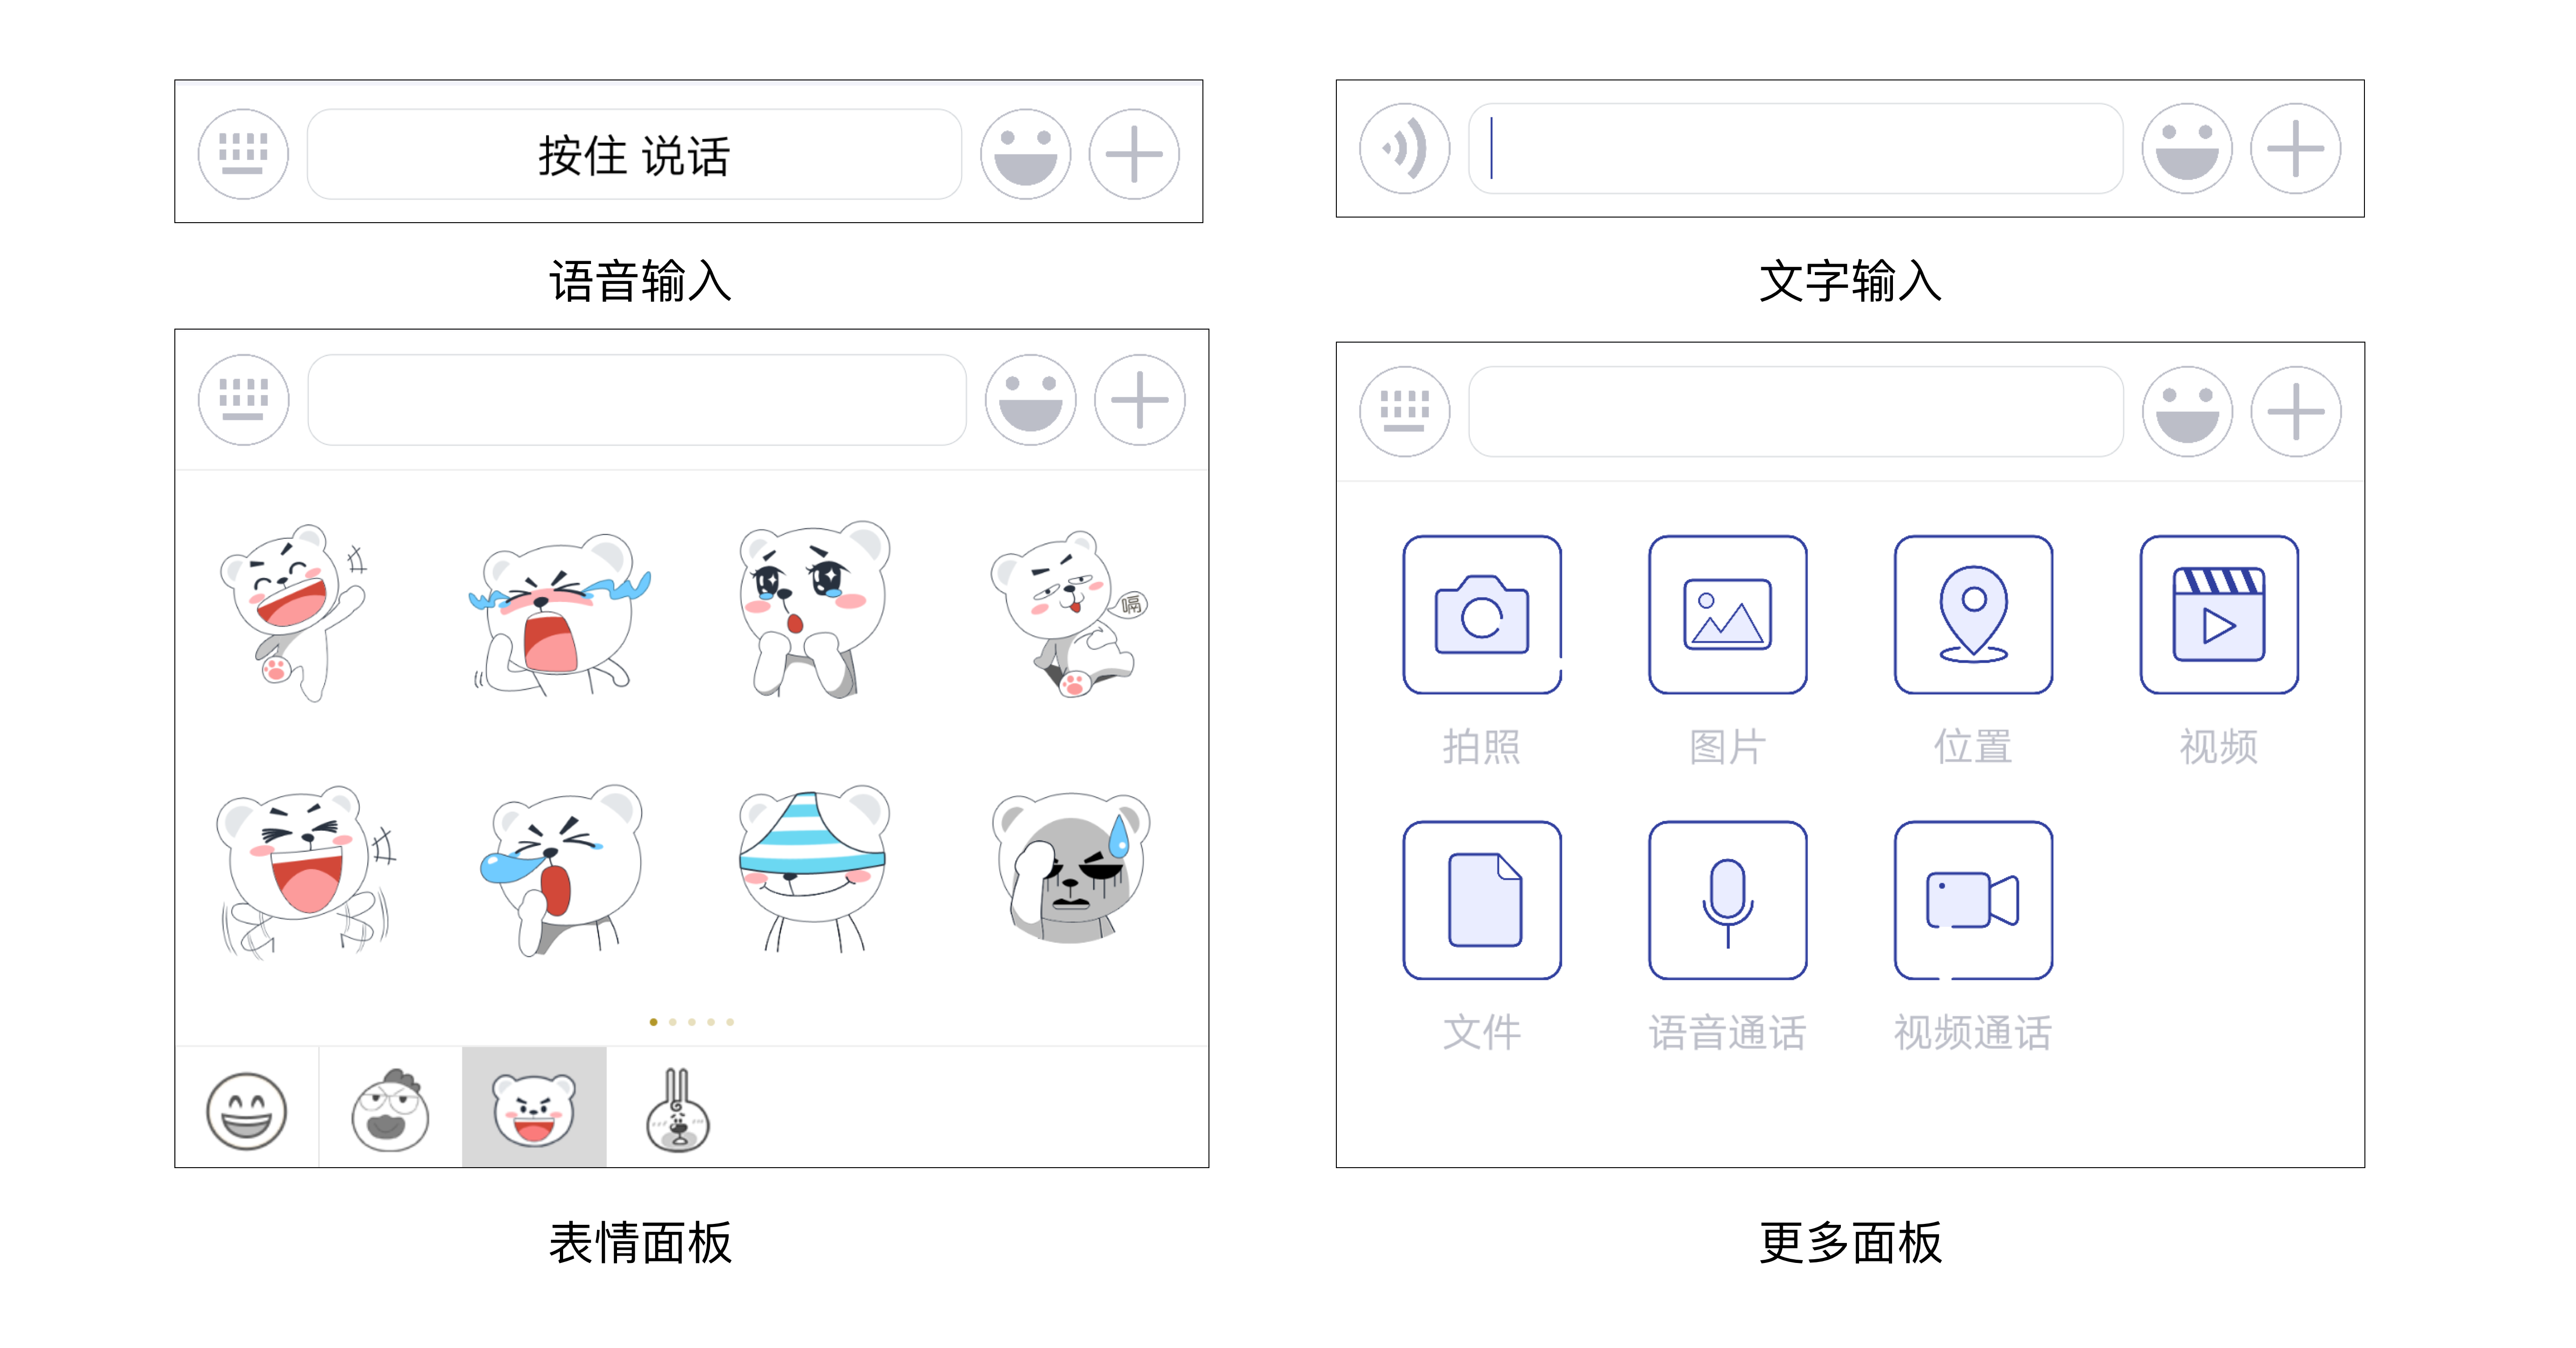
\includegraphics[width=0.95\textwidth]{images/input_panel}
		\caption{输入面板样式}
		\label{input_panel}
	\end{figure}
	
	
   	\subsubsection{表情面板的实现}
   	
   	实现省略一段文字省略一段文字省略一段文字省略一段文字省略一段文字省略一段文字省略一段文字省略一段文字省略一段文字省略一段文字省略一段文字省略一段文字省略一段文字省省略一段文字省略一段文字省略一段文字省略一段文字省略一段文字省略一段文字省略一段文字省略一段文字省略一段文字省略一段文字省略一段文字省略一段文字省略一段文字省   	
   	   	   	
   	\subsubsection{更多面板的实现}
   	
   	实现省略一段文字省略一段文字省略一段文字省略一段文字省略一段文字省略一段文字省略一段文字省略一段文字省略一段文字省略一段文字省略一段文字省略一段文字省略一段文字省省略一段文字省略一段文字省略一段文字省略一段文字省略一段文字省略一段文字省略一段文字省略一段文字省略一段文字省略一段文字省略一段文字省略一段文字省略一段文字省
   	    
   	\subsubsection{通讯录列表的实现}
   	
   	实现省略一段文字省略一段文字省略一段文字省略一段文字省略一段文字省略一段文字省略一段文字省略一段文字省略一段文字省略一段文字省略一段文字省略一段文字省略一段文字省省略一段文字省略一段文字省略一段文字省略一段文字省略一段文字省略一段文字省略一段文字省略一段文字省略一段文字省略一段文字省略一段文字省略一段文字省略一段文字省
    
	\subsubsection{埋点统计的实现}
	
	实现省略一段文字省略一段文字省略一段文字省略一段文字省略一段文字省略一段文字省略一段文字省略一段文字省略一段文字省略一段文字省略一段文字省略一段文字省略一段文字省省略一段文字省略一段文字省略一段文字省略一段文字省略一段文字省略一段文字省略一段文字省略一段文字省略一段文字省略一段文字省略一段文字省略一段文字省略一段文字省
		
          

  \subsection{表现层详细设计}
	
	  \subsubsection{Activity 基类的实现}
	  
		实现省略一段文字省略一段文字省略一段文字省略一段文字省略一段文字省略一段文字省略一段文字省略一段文字省略一段文字省略一段文字省略一段文字省略一段文字省略一段文字省省略一段文字省略一段文字省略一段文字省略一段文字省略一段文字省略一段文字省略一段文字省略一段文字省略一段文字省略一段文字省略一段文字省略一段文字省略一段文字省
	  		

	  
	  	  
	  \subsubsection{Fragment 基类的实现}
	  
		实现省略一段文字省略一段文字省略一段文字省略一段文字省略一段文字省略一段文字省略一段文字省略一段文字省略一段文字省略一段文字省略一段文字省略一段文字省略一段文字省省略一段文字省略一段文字省略一段文字省略一段文字省略一段文字省略一段文字省略一段文字省略一段文字省略一段文字省略一段文字省略一段文字省略一段文字省略一段文字省
		

  \subsection{应用层详细设计}
  	
		\subsubsection{用户系统的实现}
		
		实现省略一段文字省略一段文字省略一段文字省略一段文字省略一段文字省略一段文字省略一段文字省略一段文字省略一段文字省略一段文字省略一段文字省略一段文字省略一段文字省省略一段文字省略一段文字省略一段文字省略一段文字省略一段文字省略一段文字省略一段文字省略一段文字省略一段文字省略一段文字省略一段文字省略一段文字省略一段文字省
		
		\subsubsection{聊天功能的实现}
		
		实现省略一段文字省略一段文字省略一段文字省略一段文字省略一段文字省略一段文字省略一段文字省略一段文字省略一段文字省略一段文字省略一段文字省略一段文字省略一段文字省省略一段文字省略一段文字省略一段文字省略一段文字省略一段文字省略一段文字省略一段文字省略一段文字省略一段文字省略一段文字省略一段文字省略一段文字省略一段文字省
				
	 	\subsubsection{好友管理的实现}
	 	
	 	实现省略一段文字省略一段文字省略一段文字省略一段文字省略一段文字省略一段文字省略一段文字省略一段文字省略一段文字省略一段文字省略一段文字省略一段文字省略一段文字省省略一段文字省略一段文字省略一段文字省略一段文字省略一段文字省略一段文字省略一段文字省略一段文字省略一段文字省略一段文字省略一段文字省略一段文字省略一段文字省
	 	
		\subsubsection{群组管理的实现}
		
		实现省略一段文字省略一段文字省略一段文字省略一段文字省略一段文字省略一段文字省略一段文字省略一段文字省略一段文字省略一段文字省略一段文字省略一段文字省略一段文字省省略一段文字省略一段文字省略一段文字省略一段文字省略一段文字省略一段文字省略一段文字省略一段文字省略一段文字省略一段文字省略一段文字省略一段文字省略一段文字省
		
		\subsubsection{通讯录的实现}
		
		实现省略一段文字省略一段文字省略一段文字省略一段文字省略一段文字省略一段文字省略一段文字省略一段文字省略一段文字省略一段文字省略一段文字省略一段文字省略一段文字省省略一段文字省略一段文字省略一段文字省略一段文字省略一段文字省略一段文字省略一段文字省略一段文字省略一段文字省略一段文字省略一段文字省略一段文字省略一段文字省
		
		\subsubsection{应用列表的实现}
		
		实现省略一段文字省略一段文字省略一段文字省略一段文字省略一段文字省略一段文字省略一段文字省略一段文字省略一段文字省略一段文字省略一段文字省略一段文字省略一段文字省省略一段文字省略一段文字省略一段文字省略一段文字省略一段文字省略一段文字省略一段文字省略一段文字省略一段文字省略一段文字省略一段文字省略一段文字省略一段文字省GridView更新。
		
		\subsubsection{个人中心的实现}
		
		实现省略一段文字省略一段文字省略一段文字省略一段文字省略一段文字省略一段文字省略一段文字省略一段文字省略一段文字省略一段文字省略一段文字省略一段文字省略一段文字省省略一段文字省略一段文字省略一段文字省略一段文字省略一段文字省略一段文字省略一段文字省略一段文字省略一段文字省略一段文字省略一段文字省略一段文字省略一段文字省

 \clearpage